\section{其他方法}
\subsection{罚函数方法}
\[
    \begin{array}{rl}
        \operatorname*{min}&f(\boldsymbol{x})\\
        \mathrm{s.t.}&c_{i}(\boldsymbol{x})=0,i\in\mathcal{E}\\
        & c_{i}(\boldsymbol{x})\geqslant0,i\in\mathcal{I}
    \end{array}
\]
\begin{definition}[罚函数方法]
    罚函数方法:借助正则化技术将约束函数揉进目标函数,得到一无约束优化问题,然后极小化后者得约束函数违反度和目标函数值都尽可能小的解。
\end{definition}
\subsubsection{外点罚函数}
\[
    \min\left\{f(\boldsymbol{x})\mid c_i(\boldsymbol{x})=0,i\in\mathcal{E}\right\}
\]
\[
    \min_{\boldsymbol{x}\in \mathbb{R}^n}P(\boldsymbol{x},\pi)=f(\boldsymbol{x})+\pi\sum_{i\in\mathcal{E}}c_i^2(\boldsymbol{x})
\]
\subsection{乘子罚函数}
\begin{figure}[htbp]
    \centering
    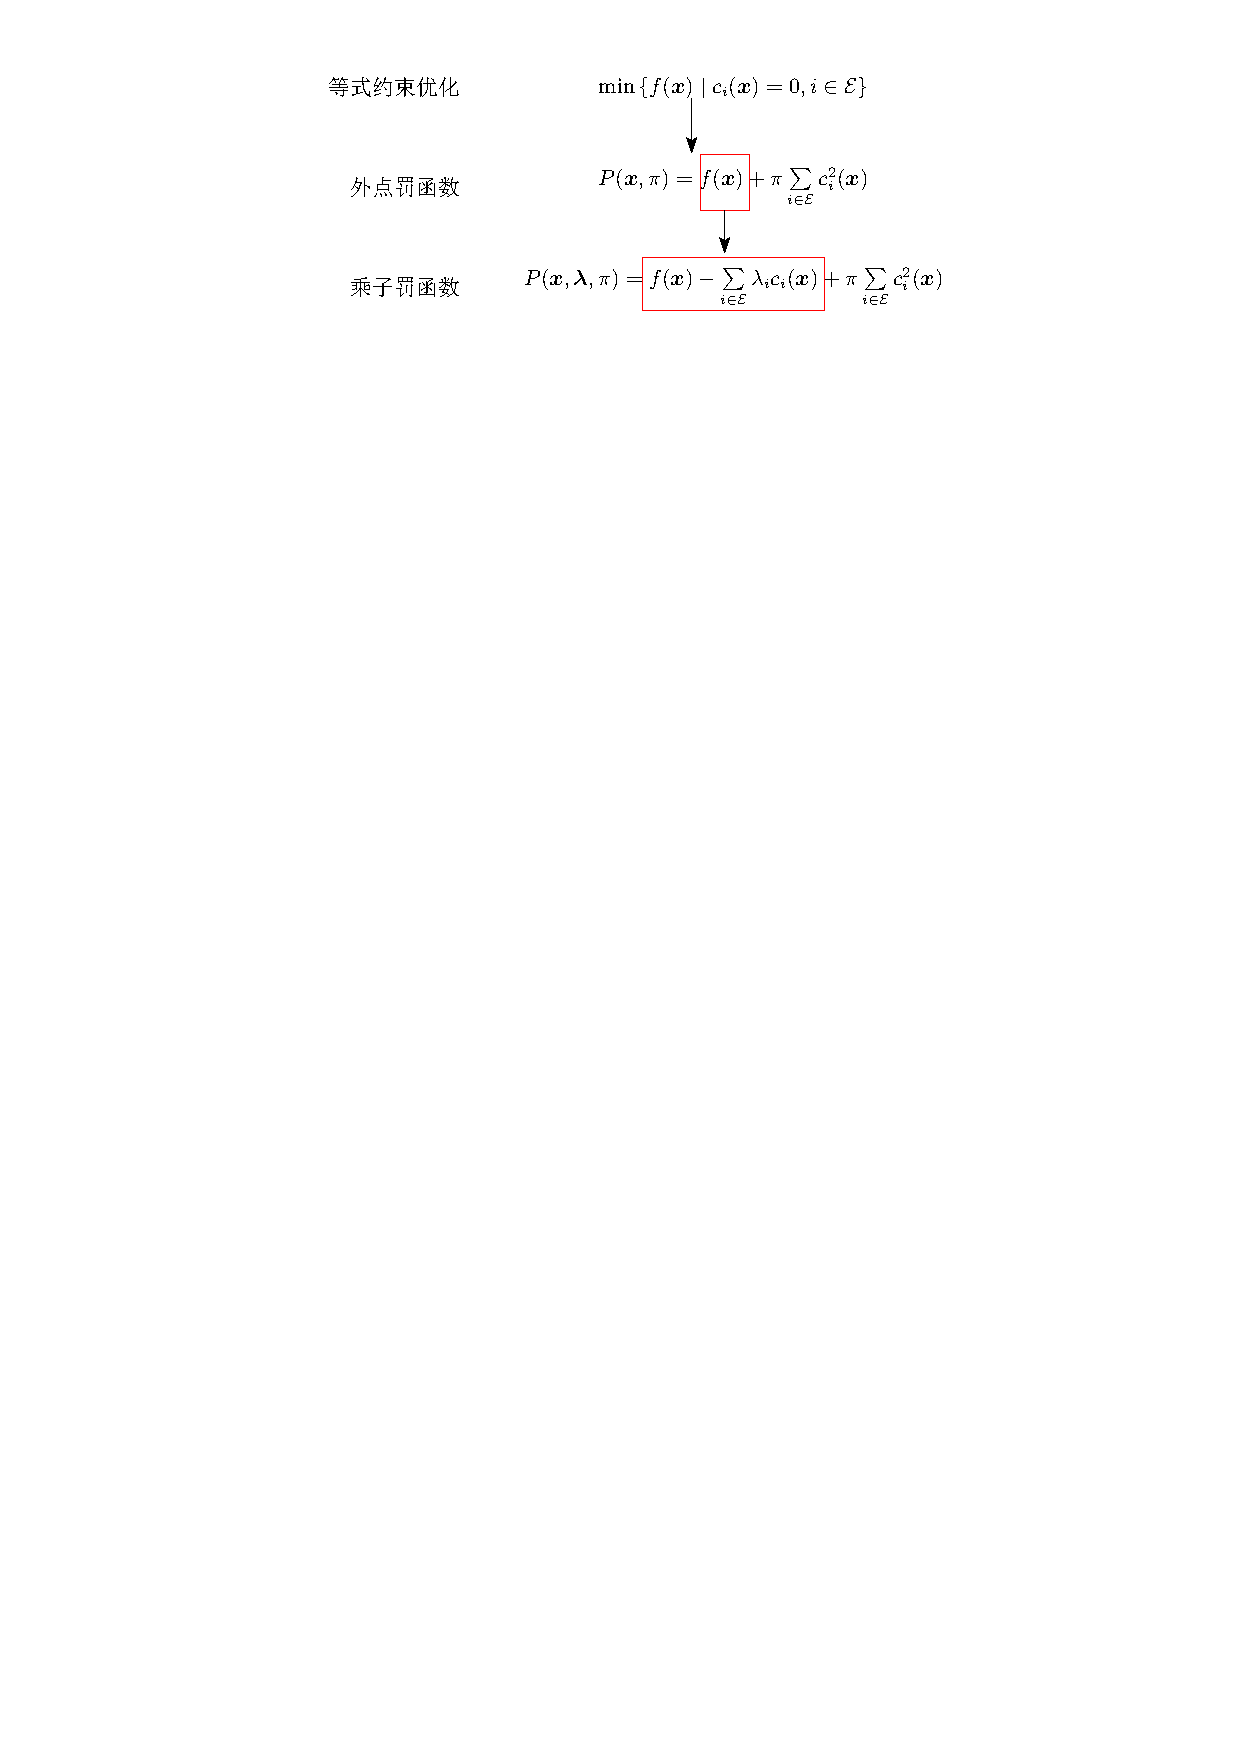
\includegraphics{image/乘子罚函数.pdf}
\end{figure}
\begin{theorem}
    设$\boldsymbol{x}^*=\arg\min\left\{f(\boldsymbol{x})\mid c_i(\boldsymbol{x})=0,i\in\mathcal{E}\right\}$,$\boldsymbol{\lambda}^*$为最优Lagrange乘子;$\nabla c_i(\boldsymbol{x}^*),i\in\mathcal{E}$线性无关。
    
    原规划问题在最优值点 $\boldsymbol{x}^*$满足二阶最优性条件。

    乘子罚函数$P(\boldsymbol{x},\boldsymbol{\lambda},\pi)=f(\boldsymbol{x})-\sum\limits_{i\in\mathcal{S}}\lambda_ic_i(\boldsymbol{x})+\pi\sum_{i\in\mathcal{S}}c_i^2(\boldsymbol{x})$ 
    
    则存在$\pi^*>0$,使对任意的$\pi\geqslant\pi^*,\boldsymbol{x}^*$为罚函数$P(\boldsymbol{x},\boldsymbol{\lambda}^*,\pi)$严格最小值点.
\end{theorem}